\documentclass[../main.tex]{subfiles}

\begin{document}
    
\subsection{Der Rohrresonator}
    \paragraph{Transferfunktion des Mikrofons}
        In \ref{fig:I_Transferfunktion} ist die Transferfunktion des Mikrofons dargestellt, die bei einer Rohrlänge von $\SI{12.5}{\milli\metre}$ aufgenommen wurde.

        \begin{figure}[H]
            \centering
            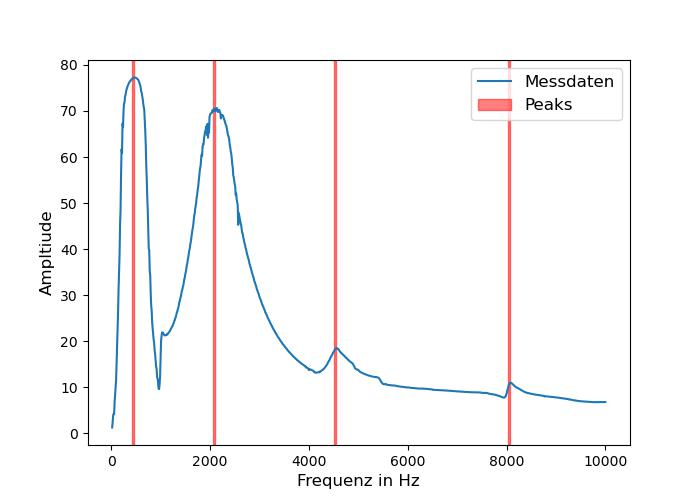
\includegraphics[width=0.8\textwidth]{Bilddateien/Auswertung/I_Transferfunktion.jpg}
            \caption{Transferfunktion des Mikrofons im Rohrresonator}
            \label{fig:I_Transferfunktion}
        \end{figure}

        Zu erkennen sind vier Maxima: $f_1=\SI{450(20)}{\hertz}$, $f_2=\SI{2090(20)}{\hertz}$, $f_3=\SI{4520(20)}{\hertz}$ und $f_4=\SI{8060(20)}{\hertz}$. Die Unsicherheit von $u=\SI{20}{\hertz}$ wurde aufgrund des Abstands der aufgenommenen Datenpunkte zueinander festgelegt. Besonders ausgeprägt sind $f_1$ und $f_2$, was in späterer Bestimmung von der Breite einiger Peaks zu beachten ist.
    
    \paragraph{Berechung der Schallgeschwindigkeit}
        \ref{fig:I_c_Resonanzspektrum} zeigt das Spektrum eines Rohresonators der Länge $\SI{60}{\centi\metre}$.

        \begin{figure}[H]
            \centering
            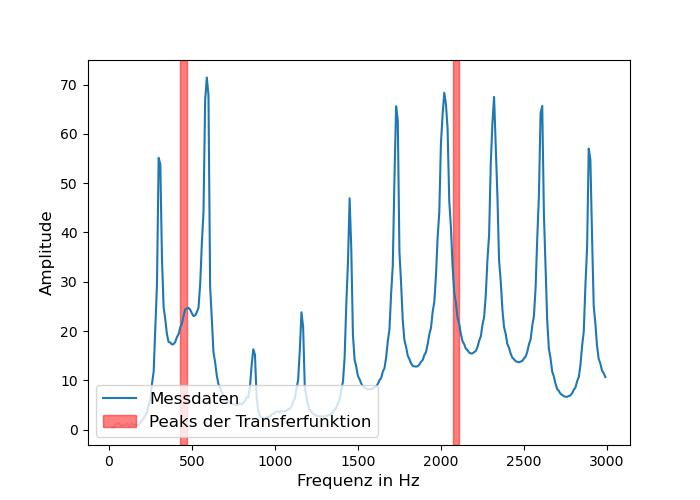
\includegraphics[width=0.8\textwidth]{Bilddateien/Auswertung/I_c_Resonanzspektrum.jpg}
            \caption{Resonanzspektrum eines 8-segmentigen Rohrers mit Segmentlänge $\SI{75}{\milli\metre}$}
            \label{fig:I_c_Resonanzspektrum}
        \end{figure}

        Zu beachten ist, dass der zweite Peak von Links ein Resultat der Transferfunktion des Mikrofons ist. Die tatsächlichen ersten 10 Resonanzen sind in Tabelle \ref{tab:I_c_Resonanzspektrum} aufgelistet.
        
        \begin{table}[H]
            \centering
            \begin{tabular}{l|l}
                \textbf{Ordnung n} & \textbf{Resonanz in Hz}\\
                \hline\hline
                $\num{1}$ & $\num{296(20)}$\\
                \hline
                $\num{2}$ & $\num{591(20)}$\\
                \hline
                $\num{3}$ & $\num{874(20)}$\\
                \hline
                $\num{4}$ & $\num{1163(20)}$\\
                \hline
                $\num{5}$ & $\num{1446(20)}$\\
                \hline
                $\num{6}$ & $\num{1741(20)}$\\
                \hline
                $\num{7}$ & $\num{2024(20)}$\\
                \hline
                $\num{8}$ & $\num{2326(20)}$\\
                \hline
                $\num{9}$ & $\num{2597(20)}$\\
                \hline
                $\num{10}$ & $\num{2898(20)}$\\
            \end{tabular}
            \caption{Resonanzfrequenzen aus \ref{fig:I_c_Resonanzspektrum}}
            \label{tab:I_c_Resonanzspektrum}
        \end{table}

        Resonanzzustände entsprechen den stehenden Wellen, welche der Randbedingung
        \begin{align}
            c = \frac{2 L\cdot f_n}{n}
            \label{eq:I_Schallgeschwindigkeit}
        \end{align}
        genügen müssen mit $c$ als Phasengeschwindigkeit, $f_n$ als Frequenz der Ordnung $n\in\N$ und $L$ als Rohrlänge. Es gilt also die lineare Relation $f_n: n\mapsto (2L/ c)\cdot n$. Ein enstprechender Fit für die Daten aus \ref{tab:I_c_Resonanzspektrum} ist in dargestellt.

        \begin{figure}[H]
            \centering
            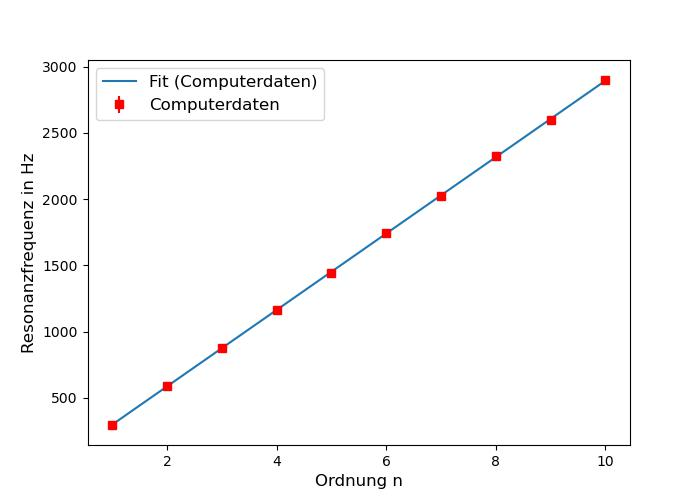
\includegraphics[width=0.8\textwidth]{Bilddateien/Auswertung/I_Schallgeschwindigkeitfit.jpg}
            \caption{linearer Fit der Resonanfrequenz in \ref{tab:I_c_Resonanzspektrum}}
            \label{fig:I_Schallgeschwindigkeitfit}
        \end{figure}

        Die Steigung der Gerade ist $a=\SI{288.5(23)}{\hertz}$ und der y-Achsenabschnitt $b=\SI{9(14)}{\hertz}$ (letzterer dient dazu, Hintergrundrauschen zu kompensieren). Mit \eqref{eq:I_Schallgeschwindigkeit} ergibt sich so $c=\SI{346.2(28)}{\metre\per\second}$. Der Literaturwert bei $\SI{20}{\celsius}$ liegt bei $c^{(lit)}=\SI{344}{\metre\per\second}$ \cite{const:sound}, was in hunder Prozent Übereinstimmumg mit dem berechneten Wert liegt.

    \paragraph{Lebensdauer von Resonanzzuständen}
        Weiter wurde ein breites Spektrum eines Rohrs der Länge $\SI{15}{\centi\metre}$ aufgenommen, um die Breite beziehungsweise Lebensdauern der Resonanzzustände zu untersuchen.

        \begin{figure}[H]
            \centering
            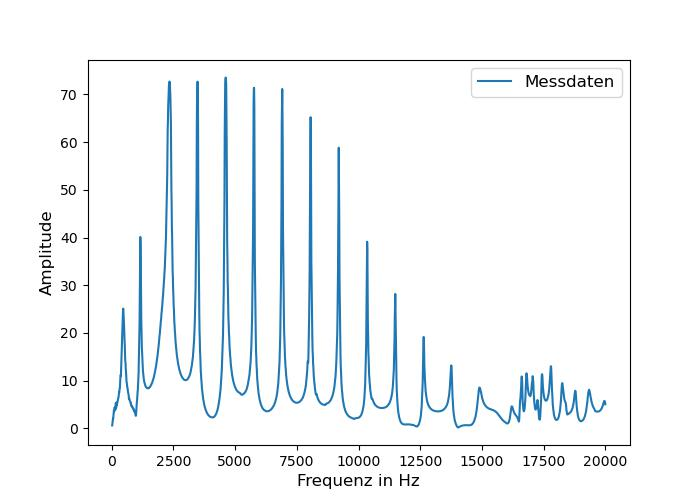
\includegraphics[width=0.8\textwidth]{Bilddateien/Auswertung/I_f_Rohspektrum.jpg}
            \caption{Spektrum eines 2-segmentigen Rohrs der Segmentlänge $\SI{75}{\milli\metre}$}
            \label{fig:I_f_Rohspektrum}
        \end{figure}

        Für einzelne Resonanzen gilt in guter Näherung die spektrale Lorentz-Auflösung 
        
        \begin{align*}
            A: \omega\mapsto \frac{K}{(\omega_0-\omega)^2 + \lambda^2},
        \end{align*}
        falls $\omega_0\gg \lambda$. Dabei ist $A(\omega)$ die Amplitude des Frequenzanteils $\omega$, $K$ die Amplitude der spektralen Auflöung, $\omega_0$ die Resoanzkreisfrequenz und $\lambda$ der Dämpfungskoeffizient.\\

        Zunächst wurden die Daten auf ein Gebiet von $\SI{5000}{\hertz}$ bis $\SI{13500}{\hertz}$ eingeschränkt, damit die Breite der Peaks weder von der Transferfunktion noch von dem chaotischen Verhalten bei hohen Frequenzen in \ref{fig:I_f_Rohspektrum} beeinflusst wird. Anschließend wurde das Spektrum in Intervalle eingeteilt, die von einem Minimum zwischen zwei Peaks zum nächsten führten. Innerhalb dieser Intervalle wurde jweils ein Lorentzfit durchgeführt, um den Einfluss von benachbarten Peaks minimal zu halten. Zuletzt wurde Gleichung für den Fit noch um eine Konstante $C\in\R$ erweitert, um störende Effekte allgemein zu berücksichtigen. Diagramm \ref{fig:I_LorentzfitVorbereitung} zeigt die Intervallhalbierung und einen exemplarischen Fit für kleine Resonanzordnung.

        \begin{figure}[H]
            \centering
            \begin{subfigure}[b]{0.8\textwidth}
                \centering
                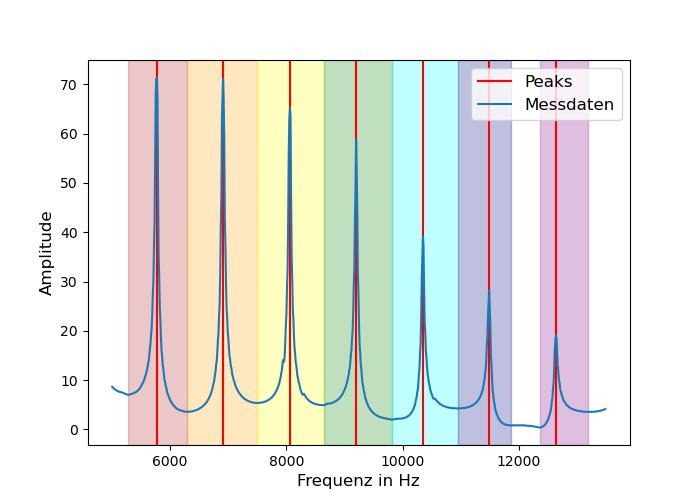
\includegraphics[width=\textwidth]{Bilddateien/Auswertung/I_f_LorentzfitVorbereitung.jpg}
                \caption{Aufteilung des Resonanzspektrums}
            \end{subfigure}
            \hfill
            \begin{subfigure}[b]{0.8\textwidth}
                \centering
                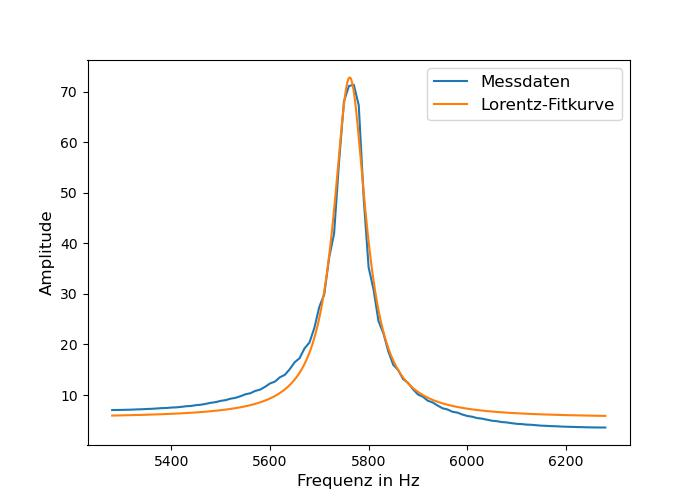
\includegraphics[width=\textwidth]{Bilddateien/Auswertung/I_f_LorentzfitBeispiel.jpg}
                \caption{Beispielhafter Lorentz-Fit eines einzelnen Peaks}
            \end{subfigure}
            \caption{Methode zum Fitten der Daten aus \ref{fig:I_f_Rohspektrum}}
            \label{fig:I_LorentzfitVorbereitung}
       \end{figure}

       In Tabelle \ref{tab:I_f_LorentzParameter} sind die Fitparameter für jeden Peak aufgeführt.

       \begin{table}[H]
        \centering
        \begin{tabular}{l|l|l|l|l}
            \textbf{Ordnung} & \textbf{Amplitude} & \textbf{Eigenfrequenz} & \textbf{Dämpfungskonstante} & \textbf{Offset}\\
            \hline
            4 & 106377(25) & 5761.6563(40) & 39.7378(60) & 5.4757(20)\\
            \hline
            5 & 117892(27) & 6908.463(40) & 42.320(60) & 4.7619(20)\\
            \hline
            6 & 83894(22) & 8057.248(40) & 37.3759(60) & 5.5416(20)\\
            \hline
            7 & 80378(25) & 9198.7491(50) & 39.9429(80) & 3.8164(20)\\
            \hline
            8 & 48372(22) & 10350.9665(70) & 37.533(20) & 3.3977(20)\\
            \hline
            9 & 38784(26) & 11483.0496(100) & 40.37(20) & 2.9755(20)\\
            \hline
            10 & 26302(27) & 12644.945(20) & 40.33(30) & 2.8268(20)
        \end{tabular}
        \caption{Fitparameter für die verschiedenen Resonanzordnungen}
        \label{tab:I_f_LorentzParameter}
    \end{table}
    
    Dass die Ordnungen bei $4$ beginnten kommt daher, dass vor ersten gefitteten Peaks bereits 4 echte Resonanzen vorhanden waren, deren Breiten aber vermutlich von der Transferfunktion verfälscht sind.\\
    
    Die Lebensdauer ergibt sich nun über $\tau=1/\lamba$ und ist in \ref{fig:I_f_Lebensdauer} zusammen mit dem Dämpfungskoeffizient visualisiert.

    \begin{figure}[H]
        \centering
        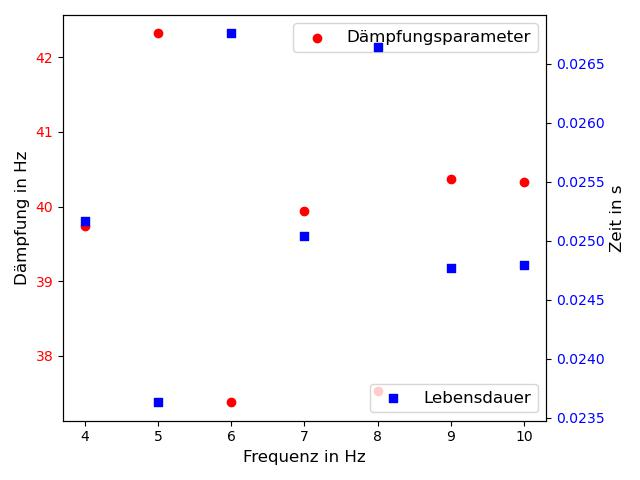
\includegraphics[width=0.8\textwidth]{Bilddateien/Auswertung/I_f_Lebensdauer.jpg}
        \caption{Dämpfungskoeffizienten aus Tabelle \ref{tab:I_f_LorentzParameter} und die zugehörige Lebensdauer aufgetragen über die Resonanzordnung}
        \label{fig:I_f_Lebensdauer}
    \end{figure}

    Es zeigt sich ein oszillatorisches Verhalten der Datenpunkte, was aber auch nur an der geringen Anzahl von Punkten liegen kann. Ein Vergleich der vierten Resonanz mit der neunten und zehnten lässt vermuten, dass die Lebensdauer aber tendenziell mit der Resonanzordnung sinkt. Dies ist vereinbar mit der Theorie des spontanten Zerfalls von quantenmechanischen, angeregten Zuständen: die Zerfallsrate steigt nämlich mit der Frequenz, also auch der Energie.

\subsection{Der Kugelresonator ohne Zwischenringe}     
    Spektrum \ref{fig:II_f_Spektren} zeigt die Resonanzen eines Kugelresonators ohne Zwischenringe, bei verschiedenen Verdrehungen von Mikrofon und Lautsprecher zueinander.
    
    \begin{figure}[H]
        \centering
        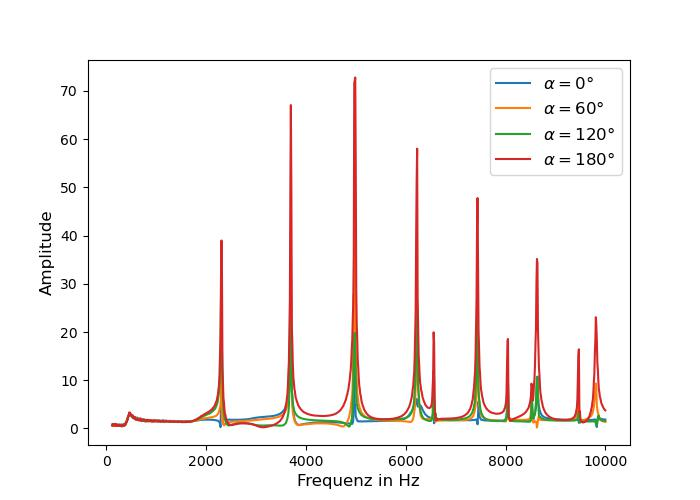
\includegraphics[width=0.8\textwidth]{Bilddateien/Auswertung/II_f_Spektren.jpg}
        \caption{Spektrum eines Kugelresonators ohne Symmetriebrüche}
        \label{fig:II_f_Spektren}
    \end{figure}

    Da die Symmetrieachse senkrecht durch den Lautsprecher (den Erzeuger der Druckmoden) verläuft, müssen auch die Kugelflächenfunktionen $Y_{m,l}$, die bis auf einen Faktor die Druckamplitude vorgeben bei dem Kugelradius, in Schieflage gesehen werden. Verdrehen der Halbkugeln zueinander variiert also sowohl den Horizontalwinkel $\varphi$, als auch den Vertikanlwinkel $\vartheta$. Im Prinzip kann so der Verlauf von $Y_{l,m}$ entlang beider Winkel gemessen werden.

    Allerdings führen die vom Lautsprecher emittierte Wellen eher zu Moden, welche entlang der Symmetrieachse eine echte Druckschwingung (d.h. mit Amplitude ungleich Null) besitzen. Dies ist gerade bei $m=0$ der Fall. Aber

    \begin{align*}
        Y_{l,m}(K(\vartheta,\varphi))\propto P_l^m(\cos(\vartheta))\cdot \exp(\cmath m\cdot\varphi)
    \end{align*}

    \noindent und $\exp(\cmath 0\cdot \varphi)=1$. Der Einfluss von $\varphi$ kann praktisch also nicht vermessen werden. ($K$ steht hier für die Konvertierungsfunkton von den Winkelkoordinaten $\vartheta,\varphi$ in kartesische Koordinaten.)\\

    Zurück zu Diagramm \ref{fig:II_f_Spektren}: die Resonanzenfrequenzen scheinen sich bei der Vedrehung der Halbkugeln nicht zu ändern, aber die Amplituden - dabei ist diese bei $\alpha=\SI{180}{\degree}$, wo sich Lautsprecher und Mikrofon gegenüberstehen, am größten. Dies stützt nochmals, dass bevorzugt Moden angeregt werden, deren Druckamplitude entlang der Symmetrieachse groß ist.

    \paragraph{Exemplarische Polschnitte}
        In \ref{fig:II_i_Polschnitte} sind die aufgenommenen Polarschnitte der Druckverteilungen aufgelistet, für die ersten vier Resonanzordnungen in \ref{fig:II_f_Spektren}. Weiterhin sind Fits der Art 
        
        \begin{align*}
            L: \vartheta\mapsto a\cdot \vert Y_{l,0}(K(\vartheta,0))\vert = a\cdot\vert P_l^0(\cos(\vartheta))\vert\footnote{\text{Es wurde $\varphi=0$ gesetzt, da für $m=0$ der Horizontalwinkel keinen Einfluss auf die Form von $Y_{l,m}$ hat.}}
        \end{align*}
        
        \noindent aufgezeigt, deren Quantenzahl $l$ den Daten am ehesten zusagt. Der Fitparameter $a$ repräsentiert den Wert der Radiallösung der Druck-Gleichung für den vorliegenden Kugelradius, sowie den Amplitudenfaktor in den Kugelflächenfunktionen selbst.

        \begin{figure}[H]
            \centering
            \begin{subfigure}[b]{0.45\textwidth}
                \centering
                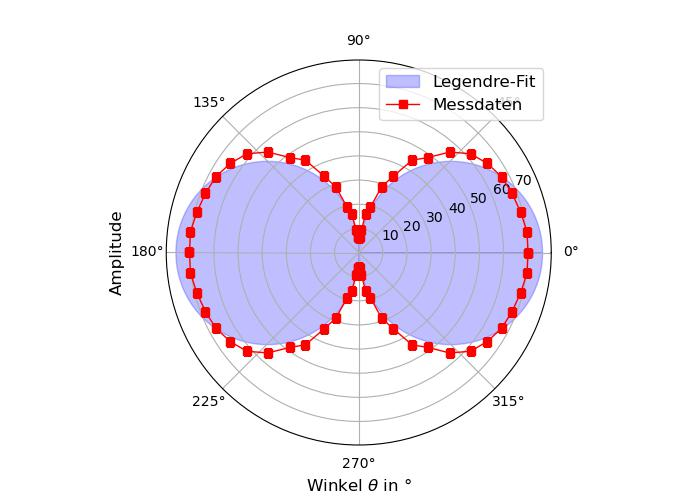
\includegraphics[width=\textwidth]{Bilddateien/Auswertung/II_i_Polschnitt_2300_10.jpg}
                \caption{Polarschnitt bei $f=\SI{2300(20)}{\hertz}$, mit Quantenzahl $l=1$}
                \label{fig:II_i_Polschnitt_2300_10}
            \end{subfigure}
            \hfill
            \begin{subfigure}[b]{0.45\textwidth}
                \centering
                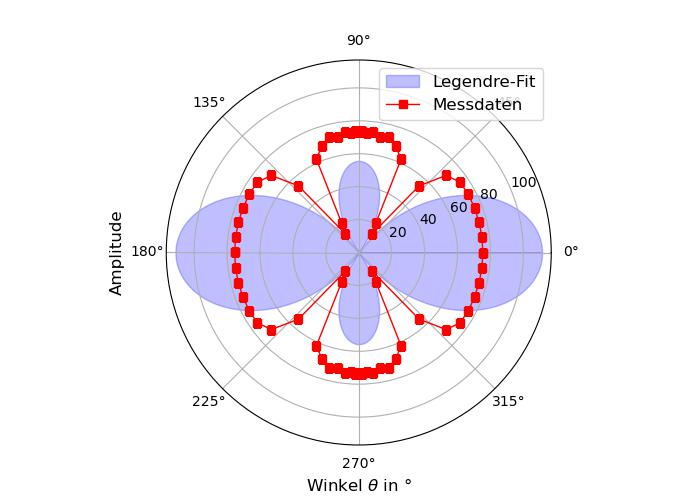
\includegraphics[width=\textwidth]{Bilddateien/Auswertung/II_i_Polschnitt_3694_20.jpg}
                \caption{Polarschnitt bei $f=\SI{3694(20)}{\hertz}$, mit Quantenzahl $l=2$}
                \label{fig:II_i_Polschnitt_3694_20}
            \end{subfigure}
            \begin{subfigure}[b]{0.45\textwidth}
                \centering
                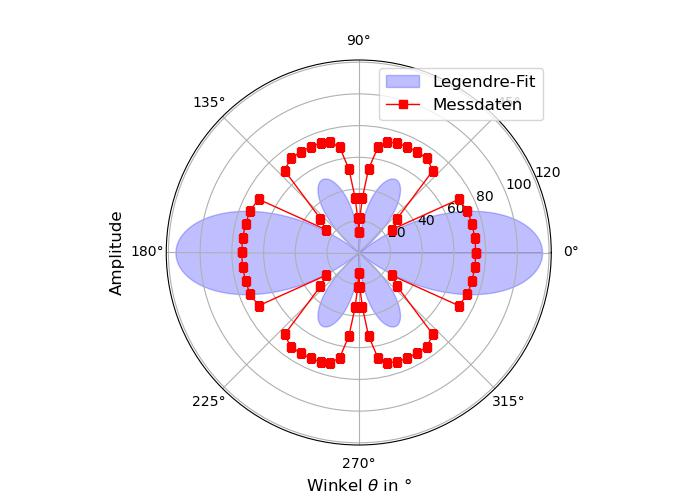
\includegraphics[width=\textwidth]{Bilddateien/Auswertung/II_i_Polschnitt_4982_30.jpg}
                \caption{Polarschnitt bei $f=\SI{4982(20)}{\hertz}$, mit Quantenzahl $l=3$}
                \label{fig:II_i_Polschnitt_4982_30}
            \end{subfigure}
            \hfill
            \begin{subfigure}[b]{0.45\textwidth}
                \centering
                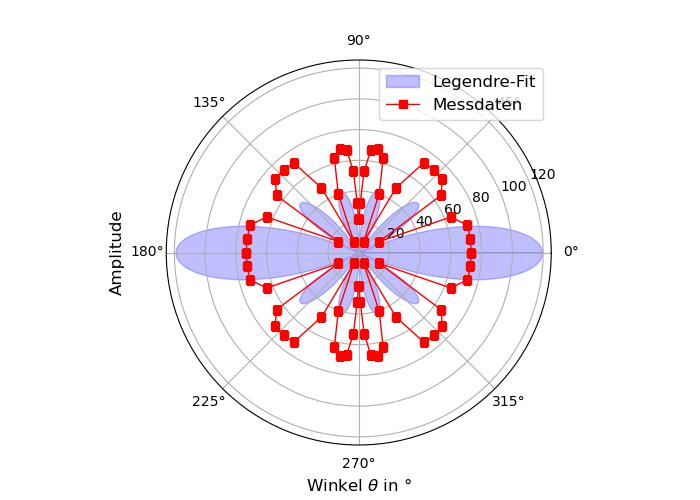
\includegraphics[width=\textwidth]{Bilddateien/Auswertung/II_i_Polschnitt_6221_50.jpg}
                \caption{Polarschnitt bei $f=\SI{6221(20)}{\hertz}$, mit Quantenzahl $l=5$}\label{fig:II_i_Polschnitt_6221_50}

            \end{subfigure}
            \caption{Polarschnitte einiger Druckverteilungen}
            \label{fig:II_i_Polschnitte}
    \end{figure}

    Bestimmt wurde die Quantenzahl $l\in\N$ je anhand der Anzahl von 'Knotenpunkten' des Polschnitts entlang der horizontalen Achse im Diagramm. Auffällig sind zwei Punkte:
    \begin{itemize}
        \item Die Polschnitte zeigen keine echten Knotenpunkte auf, sondern sind immer breiter. Dies könnte an der Entartung im Kugelresonator liegen, da ein $l$-Zustand $2l+1$ verschiedene Quantenzahlen $m\in\{-l,\hdots,l\}$ haben kann, mit gleicher Energie und somit gleicher Frequenz. Diese Zustände könnten sich also überlagern. Da aber wie besprochen, eher Zustände mit $m=0$ angeregt werden, sollte der Einfluss von diesem Umstand relativ klein sein.
        
        Ebenso könnte die Symmetriebrechung durch das Mikrofon zu der Verzerrung der Polschnitte beigetragen haben.

        \item Diagramm \ref{fig:II_i_Polschnitte} hat als Quantenzahl des viersten Polschnitts $l=5$ und nicht $l=4$ (was nach der Ordnung der Resonanzfrequenzen/ Energien zu erwarten wäre). Eine Überlagerung von Resoanzpeaks ist hier ausgeschlossen, weshalb dies sehr verwunderlich ist.
    \end{itemize}

    Die Fit-Daten sind nochmal in Tabelle \ref{tab:II_i_Polschnitte} eingetragen.

    \begin{table}[H]
        \centering 
        \begin{tabular}{l|l}
            \textbf{Polschnitt} & \textbf{Fitfunktion}\\
            \hline\hline
            \ref{fig:II_i_Polschnitt_2300_10} & $L_1: \vartheta\mapsto (\num{75.9568(40)})\cdot\vert\cos(\vartheta)\vert$\\
            \ref{fig:II_i_Polschnitt_3694_20} & $L_2: \vartheta\mapsto (\num{111.3691(50)}/2)\cdot\vert 3\cdot\cos(\vartheta)^2 - 1\vert$\\
            \ref{fig:II_i_Polschnitt_4982_30}S & $L_3: \vartheta\mapsto (\num{115.5974(50)}/2)\cdot\vert 5\cdot\cos(\vartheta)^3 - 3\cdot\cos(\vartheta)\vert$\\
            \ref{fig:II_i_Polschnitt_6221_50} & $L_5: \vartheta\mapsto (\num{119.325(60)}/8)\cdot\vert 63\cdot\cos(\vartheta)^5 - 70\cdot\cos(\vartheta)^3 + 15\cdot\cos(\vartheta)\vert$
        \end{tabular}
        \caption{Fits der Polschnitte in \ref{fig:II_i_Polschnitte}}
        \label{tab:II_i_Polschnitte}
    \end{table}

\paragraph{Doppelmaximum bei $f=\SI{5000}{\hertz}$}
    Weiter wurden die zwei Peaks bei ungefähr $f=\SI{5000}{\hertz}$ untersucht. Die Diagramme in \ref{II_i_Resonanzspektren_5000Hz} zeigen das Spektrum für verschiedene Drehwinkel der Halbkugeln.

    \begin{figure}[H]
        \centering
        \begin{subfigure}[b]{0.45\textwidth}
            \centering
            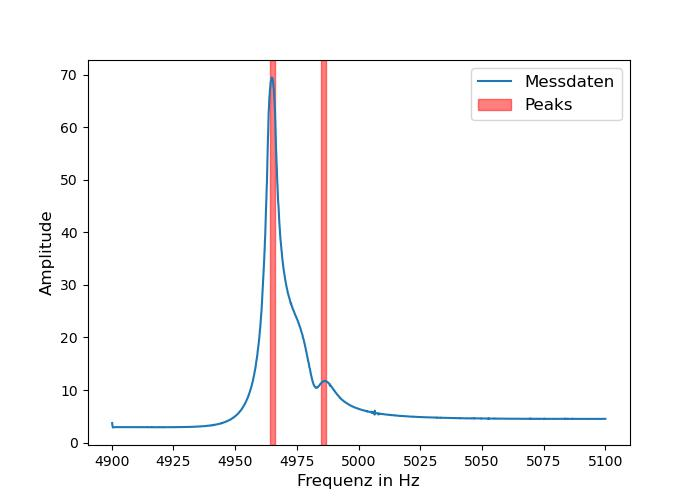
\includegraphics[width=\textwidth]{Bilddateien/Auswertung/II_i_Resonanzspektrum_0_Grad.jpg}
            \caption{Spektrum für $\alpha=\SI{0}{\degree}$}
            \label{fig:II_i_Resonanzspektrum_0_Grad}
        \end{subfigure}
        \hfill
        \begin{subfigure}[b]{0.45\textwidth}
            \centering
            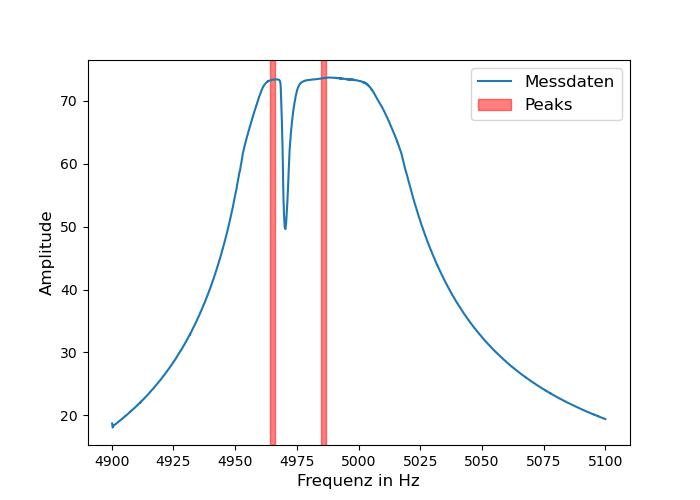
\includegraphics[width=\textwidth]{Bilddateien/Auswertung/II_i_Resonanzspektrum_90_Grad.jpg}
            \caption{Spektrum für $\alpha=\SI{90}{\degree}$}
            \label{fig:II_i_Resonanzspektrum_90_Grad}
        \end{subfigure}
        \begin{subfigure}[b]{0.45\textwidth}
            \centering
            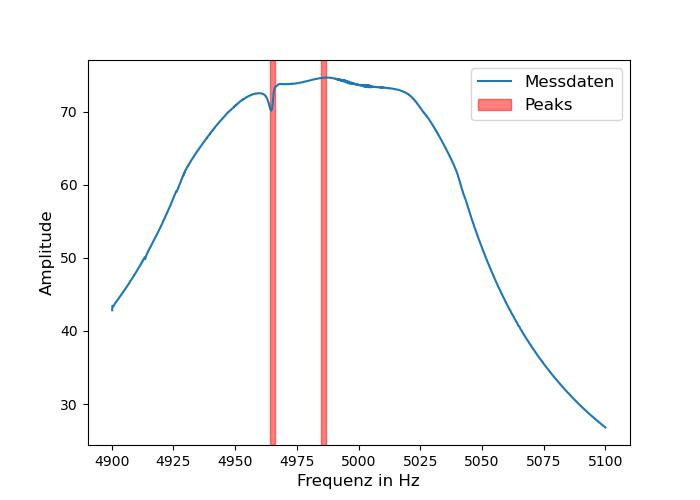
\includegraphics[width=\textwidth]{Bilddateien/Auswertung/II_i_Resonanzspektrum_180_Grad.jpg}
            \caption{Spektrum für $\alpha=\SI{180}{\degree}$}
            \label{fig:II_i_Resonanzspektrum_180_Grad}
        \end{subfigure}
        \caption{Resonanzspektren der Peaks des Kugelresonators bei $f_1=\SI{4965(20)}{\hertz}$ und $f_2=\SI{4986(20)}{\hertz}$}
        \label{fig:II_i_Resonanzspektren_5000Hz}
    \end{figure}

    Es ist eine starke Abhängigkeit der Peakbreite von dem Drehwinkel zu erkennen, die sich auch bei den Polschnitten in \ref{fig:II_j_Polschnitte_5000} wiederspiegelt.

    \begin{figure}[H]
        \centering
        \begin{subfigure}[b]{0.45\textwidth}
            \centering
            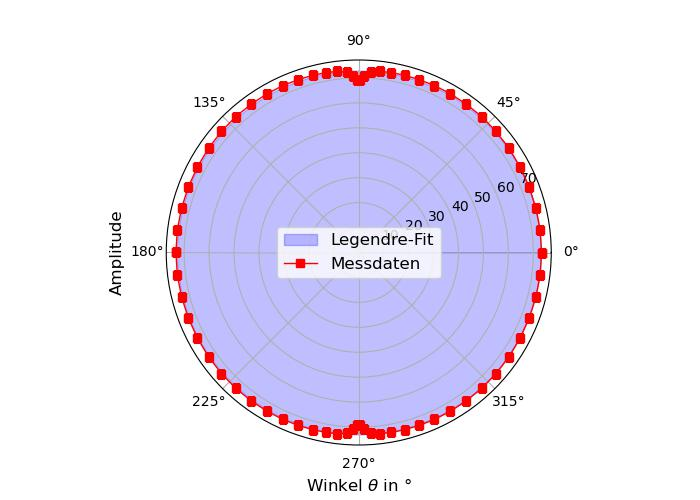
\includegraphics[width=\textwidth]{Bilddateien/Auswertung/II_j_Polschnitt_4965_00.jpg}
            \caption{Polarschnitt bei $f=\SI{4965(20)}{\hertz}$, mit Quantenzahl $l=0$}
            \label{fig:II_j_Polschnitt_4965_00}
        \end{subfigure}
        \hfill
        \begin{subfigure}[b]{0.45\textwidth}
            \centering
            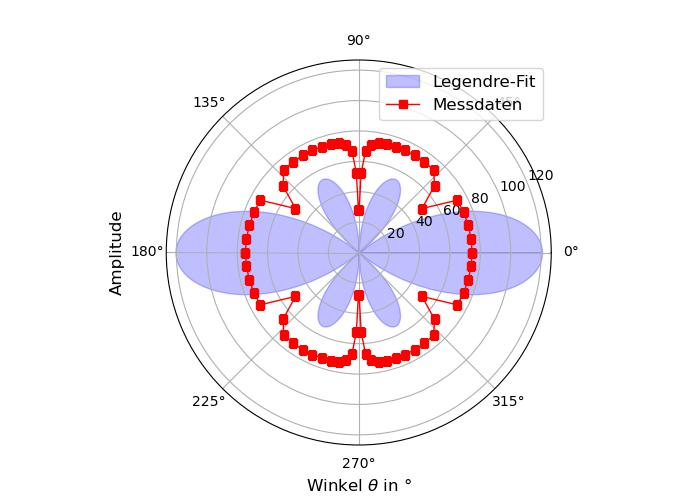
\includegraphics[width=\textwidth]{Bilddateien/Auswertung/II_j_Polschnitt_4986_30.jpg}
            \caption{Polarschnitt bei $f=\SI{4986(20)}{\hertz}$, mit Quantenzahl $l=3$}
            \label{fig:II_j_Polschnitt_4986_30}
        \end{subfigure}
        \caption{Polarschnitte weiterer Druckverteilungen bei einer Verdrehung von $\alpha=\SI{180}{\degree}$ beider Halbkugeln zueinander}
        \label{fig:II_j_Polschnitte_5000}
    \end{figure}

    Zu erwarten wären Quantenzahlen um $l=3$ herum gewesen, da die Resonanzfrequenzen recht nahe der bei \ref{fig:II_i_Polschnitt_4982_30} liegen. Ebenfalls wäre zu erwarten gewesen, das die Quantenzahl $m$ hier ungleich Null ist, da bei der genauen Messsung trotz Entartung, wegen kleiner Symmetriebrüche eine Aufspaltung der Zustand beobachtbar sein könnte.\\

    Der Schnitt \ref{fig:II_j_Polschnitt_4986_30} ähnelt \ref{fig:II_i_Polschnitt_4982_30} recht stark und erfüllt die Erwartungen. Auf \ref{fig:II_j_Polschnitt_4965_00} trifft dies nicht zu. Vermutlich sorgte die hohe Winkelabhängigkeit der Peakbreite für diese Verzerrung. Eine alternative Erklärung ist, dass der Zustand in \ref{fig:II_j_Polschnitt_4965_00} zu einer anderen Hauptquantenzahl $n\in\N$ gehört.

\subsection{Der Kugelresonator mit Zwischenringen}        
    Für diese Sektion wird der Kugelresonator mit einem Zwischenring der Dicke $d=\SI{9}{\milli\metre}$ betrachtet. Dadurch verläuft die Symmetrieachse nun näherungsweise senktrecht durch das Zentrum der oberen und unteren Halbkugel, und nicht mehr durch den Lautsprecher. Eine Verdrehung der Halbkugeln entspricht also einer Variation des Horizontalwinkels $\varphi$, $\vartheta$ bleibt konstant gleich $\vartheta_0\in(0,\pi)$. Diagramm \ref{fig:III_l_Vergleichspektrum} zeigt das Spektrum des Resonators im Vergleich zu dem ohne Zwischenring.

    \begin{figure}[H]
        \centering
        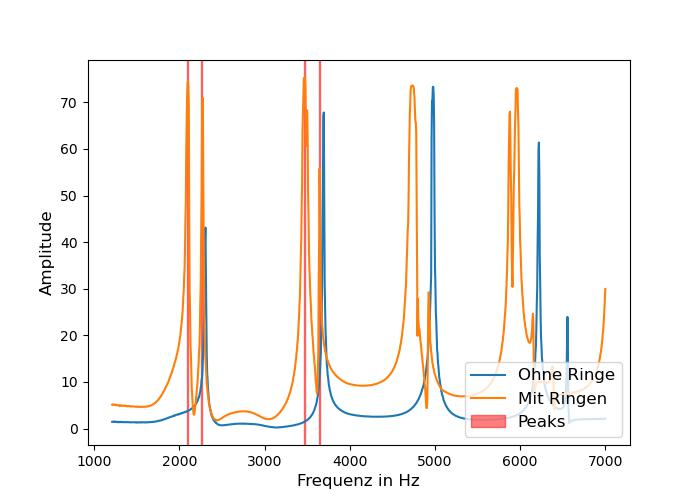
\includegraphics[width=0.8\textwidth]{Bilddateien/Auswertung/III_l_Vergleichspektrum.jpg}
        \caption{Spektrum des Kugelresonators mit und ohne Zwischenring}
        \label{fig:III_l_Vergleichspektrum}
    \end{figure}

    Das Einsetzen des Zwischenrings sorgt also für die Aufspaltung der Peaks in gebündelte Peak-Gruppen. Dies stimmt mit der Theorie überein, nach der ein Symmetriebruch des Systems die Entartung der Zustände für ein festes $l\in\N$ aufhebt (die verschiedenen Formen der Kugelflächenfunktionen bei anderen $m\in\N$ sorgen für eine je andere Resonanzenergie) Für eine genauere Betrachtung ist in Diagramm \ref{III_l_Vergleichspektrum_Nahaufnahme} eine Nahaufnahme abgebildet.

    \begin{figure}[H]
        \centering
        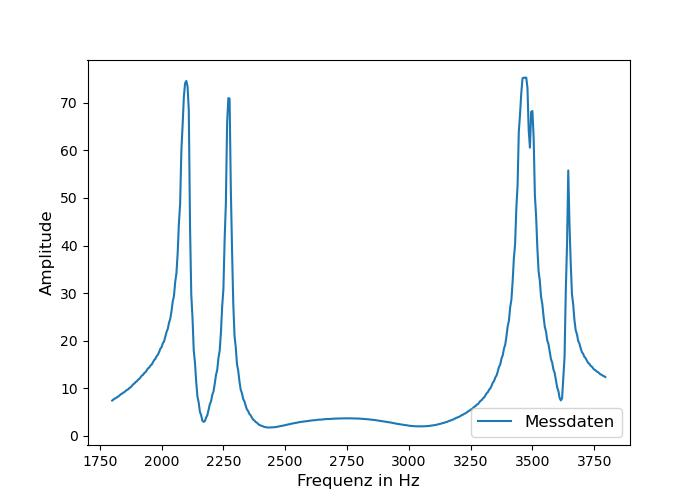
\includegraphics[width=0.8\textwidth]{Bilddateien/Auswertung/III_l_Vergleichspektrum_Nahaufnahme.jpg}
        \caption{Spektrum des Kugelresonators mit und ohne Zwischenring}
        \label{fig:III_l_Vergleichspektrum_Nahaufnahme}
    \end{figure}

    Der erste Peak in \ref{fig:III_l_Vergleichspektrum} spaltet sich also in zwei Peaks auf, und der zweite in drei. Theoretisch sollte die $2l+1$-fache Entartung, auf eine $l+1$-fache redzuiert werden. Dies kommt daher, dass die Kugelflächenfunktionen zu $-m,m$ sich nur in der Phase und Ampltiude unterscheiden. Denn die Legrende-Polynome $P_l^m$ und $P_l^{-m}$ sind identitisch bis auf einen Zahlenfaktor. Eine Gruppe von zwei Peaks, heißt also $2=l_1+1$, also $l_1=1$. Analog folgt für drei Peaks $l_2=2$. Diese Quantenzahlen stimmen mit denen der Polschnitte \ref{fig:II_i_Polschnitt_2300_10} und \ref{fig:II_i_Polschnitt_3694_20} überein.

    \paragraph{Exemplarische Azimutalschnitte}
        Darstellung \ref{fig:III_jk_Azimutalschnitte} zeigt einige Azimutalschnitte der Druckverteilungen auf der Kugeloberfläche. Da der Winkel $\vartheta$ nicht verändert wird und immer eine Überlagung von Resonanzen mit $m,-m$ betrachtet wird, eignet sich zudem ein Fit der Form 
        \begin{align*}
            L'_{\PM}: \varphi\mapsto \alpha'\cdot\vert Y_{l,0}(\vartheta_0,\varphi)\pm \vert Y_{l,0}(\vartheta_0,\varphi)\vert =: a'\cdot\vert\cos(m\varphi)\vert\footnote{\text{testest}}
        \end{align*}

        \begin{figure}[H]
            \centering
            \begin{subfigure}[b]{0.45\textwidth}
                \centering
                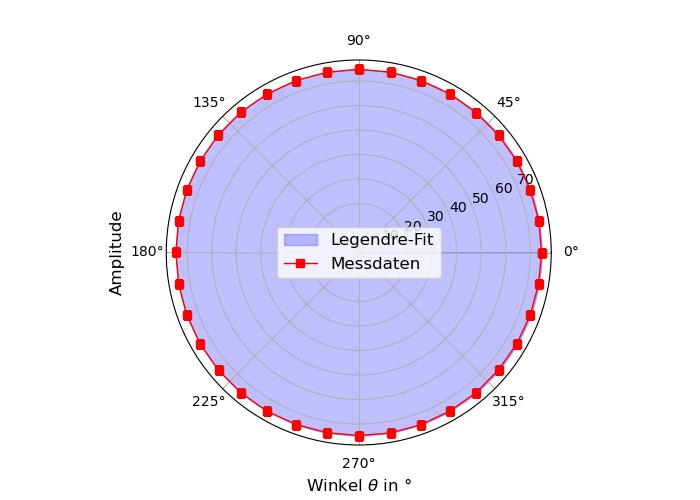
\includegraphics[width=\textwidth]{Bilddateien/Auswertung/III_jk_Polschnitt_2093_0.jpg}
                \caption{Azimutalschnitt bei $f=\SI{2300(20)}{\hertz}$, mit Quantenzahlen $l=1, m=0$}
                \label{fig:III_jk_Polschnitt_2093_0}
            \end{subfigure}
            \hfill
            \begin{subfigure}[b]{0.45\textwidth}
                \centering
                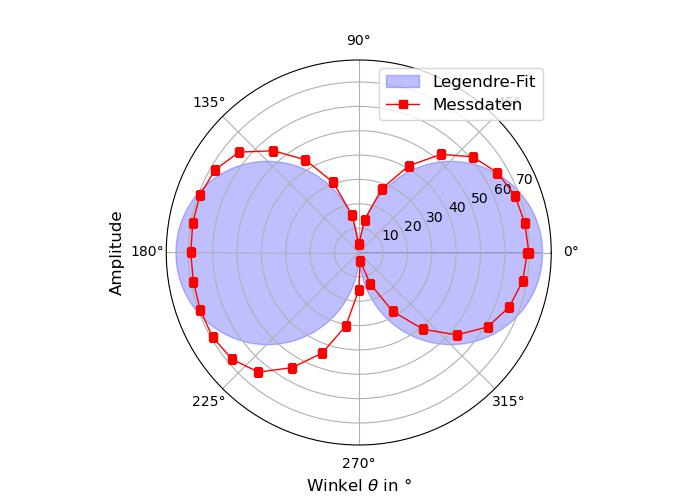
\includegraphics[width=\textwidth]{Bilddateien/Auswertung/III_jk_Polschnitt_2263_1.jpg}
                \caption{Azimutalschnitt bei $f=\SI{3694(20)}{\hertz}$, mit Quantenzahlen $l=1, m=1$}
                \label{fig:III_jk_Polschnitt_2263_1}
            \end{subfigure}
            \begin{subfigure}[b]{0.45\textwidth}
                \centering
                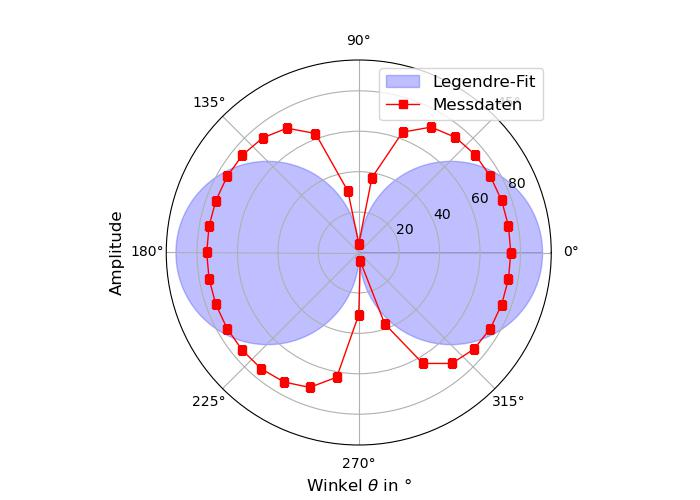
\includegraphics[width=\textwidth]{Bilddateien/Auswertung/III_jk_Polschnitt_3464_1.jpg}
                \caption{Azimutalschnitt bei $f=\SI{4982(20)}{\hertz}$, mit Quantenzahlen $l=2, m=1$}
                \label{fig:III_jk_Polschnitt_3464_1}
            \end{subfigure}
            \hfill
            \begin{subfigure}[b]{0.45\textwidth}
                \centering
                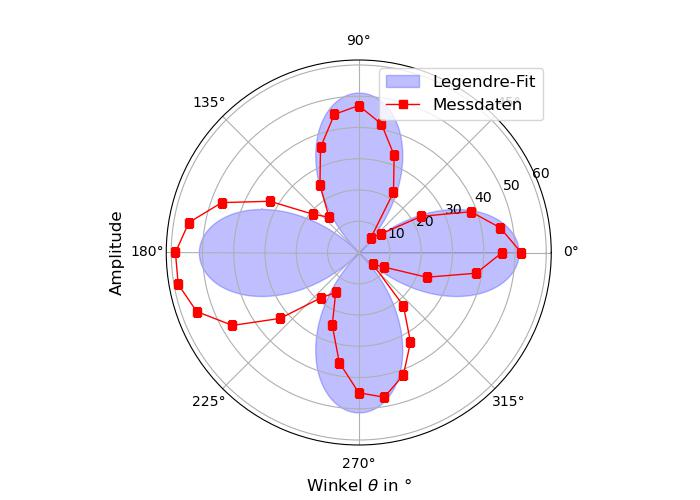
\includegraphics[width=\textwidth]{Bilddateien/Auswertung/III_jk_Polschnitt_3645_2.jpg}
                \caption{Azimutalschnitt bei $f=\SI{6221(20)}{\hertz}$, mit Quantenzahlen Quantenzahlen $l=2, m=2$
                }\label{fig:III_jk_Polschnitt_3645_2}

            \end{subfigure}
            \caption{Azimutalschnitt einiger Druckverteilungen}
            \label{fig:III_jk_Azimutalschnitte}
        \end{figure}

        Im Allgemeinen zeigt sich eine gute qualitative Übereinstimmumg von Fits und Datenpunkten. Auch die Quantenzahl $l=1$ bei \ref{fig:III_jk_Polschnitt_2093_0}, \ref{fig:III_jk_Polschnitt_2263_1} und $l=2$ bei \ref{fig:III_jk_Polschnitt_3464_1}, \ref{fig:III_jk_Polschnitt_3645_2} bestätigt die Vermutungen anhand von Spektrum \ref{fig:III_l_Vergleichspektrum_Nahaufnahme}. Ein dritter Polschnitt für $l=2$ wurde allerdings nicht aufgenommen, weil der dritte Peak wegen der geringen Auflösung am Versuchstag nicht bemerkt wurde.\\

        In Tabelle \ref{tab:III_jk_Azimutalschnitte} sind alle relevanten Fit-Daten aufgeführt.

        \begin{table}[H]
            \centering
                \begin{tabular}{l|l}
                    \textbf{Azimutalschnitt} & \textbf{Fitfunktion}\\
                    \hline\hline
                    \ref{fig:III_jk_Polschnitt_2093_0} & $L'_{1,0}: \varphi\mapsto 74.6608(30)$\\
                    \ref{fig:III_jk_Polschnitt_2093_0} & $L'_{1,1}: \varphi\mapsto (75.2712(40))\cdot\vert\cos(\varphi)\vert$\\
                    \ref{fig:III_jk_Polschnitt_2093_0} & $L'_{2,1}: \varphi\mapsto (90.7064(40))\cdot\vert\cos(\varphi)\vert$\\
                    \ref{fig:III_jk_Polschnitt_2093_0} & $L'_{2,2}: \varphi\mapsto (51.1803(40))\cdot\vert\cos(2\varphi)\vert$
                \end{tabular}
                \caption{Fits der Azimutalschnitte in \ref{fig:III_jk_Azimutalschnitte}}
                \label{tab:III_jk_Azimutalschnitte}
        \end{table}

    \paragraph{Untersuchung der Frequenzaufspaltung}
        Es wird nun der quantitative Einfluss der Zwischenringdicke auf die Aufspaltung eines Peaks in mehrere diskutiert. Hierfür wurde ein Spektrum \ref{fig:III_n_Ringdickenspektrum} für verschiedene Ringdicken aufgenommen.
        
        \begin{figure}[H]
            \centering
            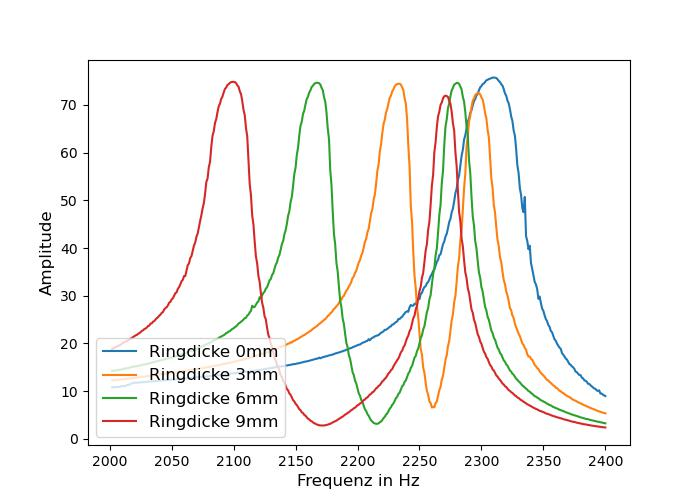
\includegraphics[width=0.8\textwidth]{Bilddateien/Auswertung/III_n_Ringdickenspektrum.jpg}
            \caption{Aufspaltung des Resonanzpeaks bei $f=\SI{2300(20)}{\hertz}$ durch verschiedene Zwischenringe}
            \label{fig:III_n_Ringdickenspektrum}
        \end{figure}

        Zum einen scheint bei höherer Ringdicke eine immer stärkere Frequenzaufspaltung vorzuliegen, zum anderen geschieht allgemein eine Frequenzverschiebung nach links. Dies heißt also, dass eine stärkere Symmetriebrechung die Energie stationärer Zustände verringert. 
        
        In Diagramm ist die Frequenzaufspaltung nochmals 
        über die Ringdicke aufgetragen. Es lässt sich ein linearer Zusammenhang vermuten, deshalb wurde auch ein linearer Fit durchgeführt. Es liegt also eine Ähnlichkeit zum Beispiel zum normalen Zeeman-Effekt vor, der eine Symmetriebrechung entlang der Feldachse bewirkt. Dort kommt es ebenso zu einer lineare Aufspaltung für quantenmechanische Zustände bewirkt. Allerdings ist dort keine allgemeine Frequenzverschiebung gegeben.

        \begin{figure}[H]
            \centering
            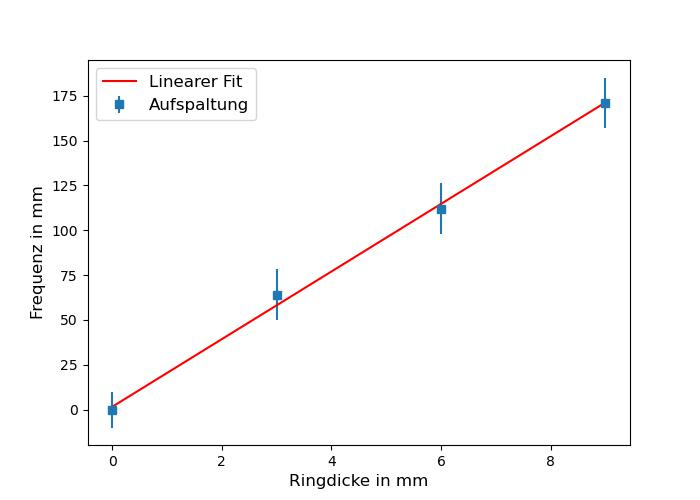
\includegraphics[width=0.8\textwidth]{Bilddateien/Auswertung/III_n_Frequenzaufspaltung.jpg}
            \caption{Die Frequenzaufspaltung in \ref{fig:III_n_Ringdickenspektrum} aufgetragen gegen die Rindicke}
            \label{fig:III_n_Frequenzaufspaltung}
        \end{figure}

        Die Steigung beträgt $\SI{18.9(19)}{\hertz\per\milli\metre}$, der y-Achsenabschnitt $\SI{2(10)}{\hertz}$. Letzter ist im Rahmen der Unsicherheit Null, da ohne Ring auch keine Frequenzaufspaltung auftrifft.

\subsection{Das Wasserstofmolekül}
    In diesem Abschnitt werden die Ergebnisse zu den mit Blenden gekoppelten Kugelresonatoren untersucht. Zunächst zeigt Diagramm \ref{fig:IV_Transferfunktion} die Transferfunktion der Kugelresonatoren.

    \begin{figure}[H]
        \centering
        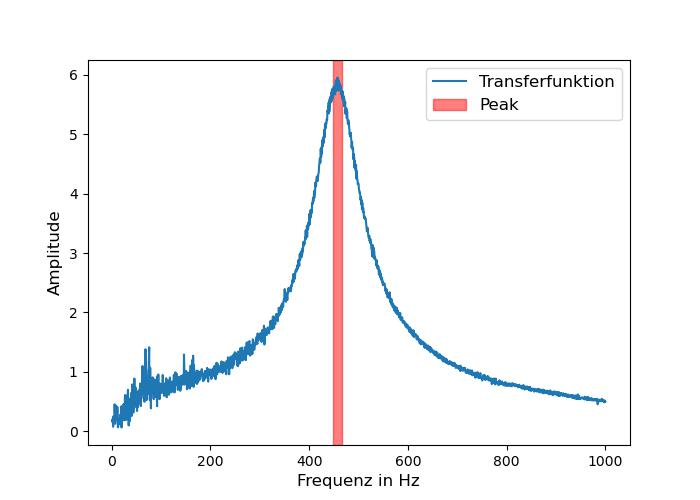
\includegraphics[width=0.8\textwidth]{Bilddateien/Auswertung/IV_Transferfunktion.jpg}
        \caption{Transferfunktion der gekoppelten Kugelresonatoren}
        \label{fig:IV_Transferfunktion}
    \end{figure}

    Es ist ein einzelner, aber breiter Peak bei $f=\SI{458(10)}{\hertz}$ zu erkennen. Abbildung \ref{fig:IV_a_Spektren} bestätigt, dass es sich hier in der Tat um die Transferfunktion handelt und um keine Resonanz: alle dort abgebildeten Peaks haben einen kleinen Buckel ungefähr bei $f$, der nicht auf die verschiedenen Kopplungsgrade reagiert.
    
    
    \paragraph{$1\sigma$-Molekülorbitale}
        Abbildung zeigt zunächst das niedere Resonanzspektren bei mehreren Blendenöffnungen.

        \begin{figure}[H]
            \centering
            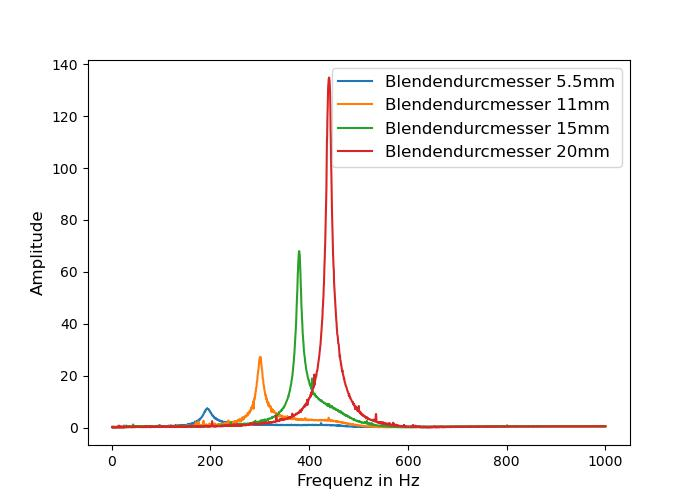
\includegraphics[width=0.8\textwidth]{Bilddateien/Auswertung/IV_a_Spektren.jpg}
            \caption{Der erste Resonanzpeak zwei gekoppelter Kugelresonatoren }
            \label{fig:IV_a_Spektren}
        \end{figure}

        Dass sowohl Amplitude als auch Frequenz der Resonanz bei einen weiteren Blendenöffnung größer werden, hat denselben Grund. Durch die größere Öffnung gelangen mehr elementare Druckwellen von einem Kugelresonator in den anderen. Durch die Überlagerungen dieser wird die Druckschwingung stärker und geht auch schneller von statten: dies resultiert in einer höheren Amplitude und kinetischen Energie der Luft (also auch einer höheren Energie der Druckmode).\\
        
        In Anologie zu den quantenmechanischen Molekülorbitalen kann nun anhand der Phasenverschiebung der Welle in Lautsprecher und Mikrofon festgestellt werden, ob der Zustand bindend oder antibindend ist. Eine Verschiebung von $\SI{180}{\degree}$ liegt bei antibindenden 
        Zuständen vor, eine von $\SI{0}{\degree}$ bei bindenden. Diagramm zeigt die releveanten Phasen bei der größten Blendenöffung und einen Verdrillwinkel von $\alpha=\SI{180}{\degree}$ zwischen Lautsprecher und Mikrofon.

        \begin{figure}[H]
            \centering
            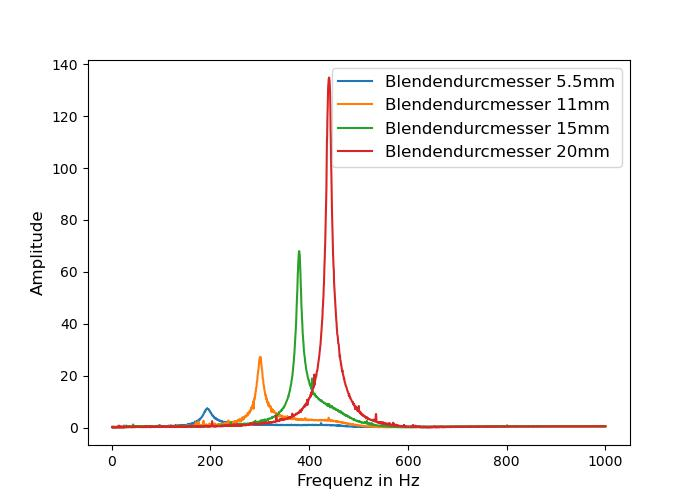
\includegraphics[width=0.8\textwidth]{Bilddateien/Auswertung/IV_a_Spektren.jpg}
            \caption{Der erste Resonanzpeak zwei gekoppelter Kugelresonatoren }
            \label{fig:IV_a_Spektren}
        \end{figure}


\subsection{Der Rohresonator mit Blenden}
    \paragraph{Tight-Binding-Methode}
        \begin{figure}[H]
            \centering
            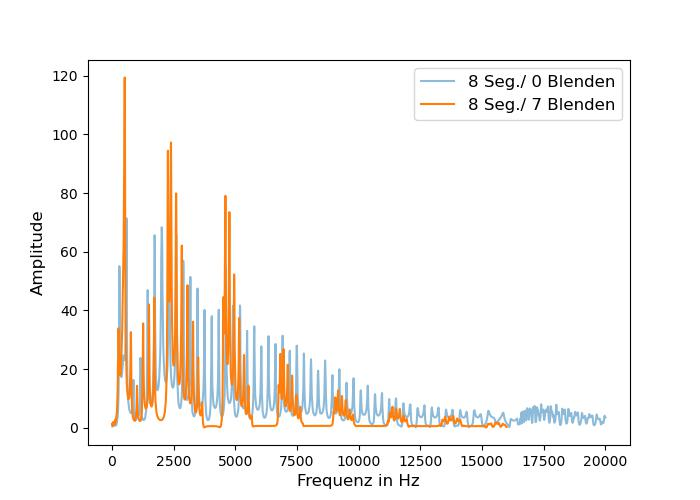
\includegraphics[width=0.8\textwidth]{Bilddateien/Auswertung/V_i_Resonanzspektrum_Lang.jpg}
            \caption{Resonanzspektrum eines 8-segmentigen Rohrs der Segmentlänge $\SI{75}{\milli\metre}$, einmal mit sieben Blenden und einmal ohne}
            \label{fig:V_i_Resonanzspektrum_Lang}
        \end{figure}

        \begin{figure}[H]
            \centering
            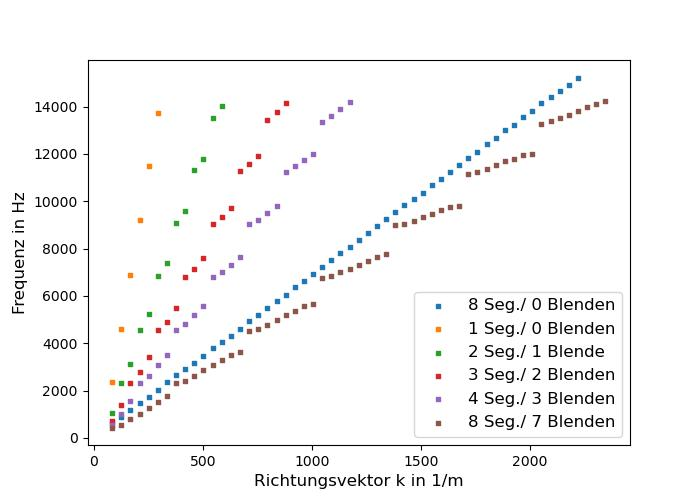
\includegraphics[width=0.8\textwidth]{Bilddateien/Auswertung/V_j_Dispersionsrelation_Lang.jpg}
            \caption{Dispersionsrelation der Resonanzspektren des Rohrs aus \ref{fig:V_i_Resonanzspektrum_Lang}, für verschiedene Segment- und Blendenzahlen}
            \label{fig:V_j_Dispersionsrelation_Lang}
        \end{figure}


    \paragraph{Schwaches periodisches Potential}
        \begin{figure}[H]
            \centering
            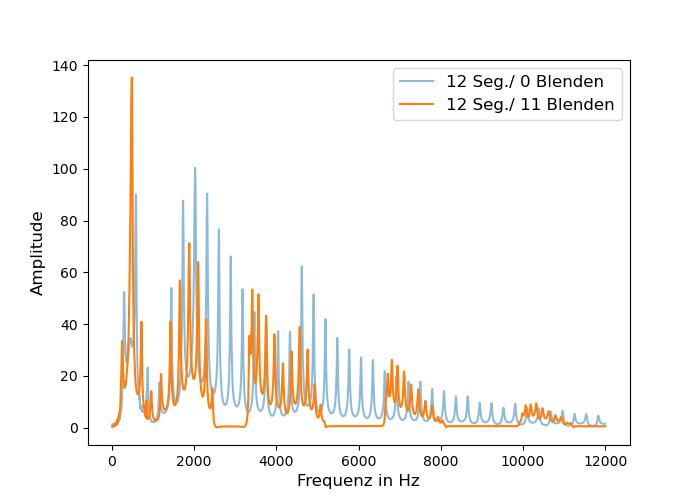
\includegraphics[width=0.8\textwidth]{Bilddateien/Auswertung/V_l_Resonanzspektrum_Kurz.jpg}
            \caption{Resonanzspektrum eines 12-segmentigen Rohrs der Segmentlänge $\SI{50}{\milli\metre}$, einmal mit sieben Blenden und einmal ohne}
            \label{fig:V_l_Resonanzspektrum_Kurz}
        \end{figure}

        \begin{figure}[H]
            \centering
            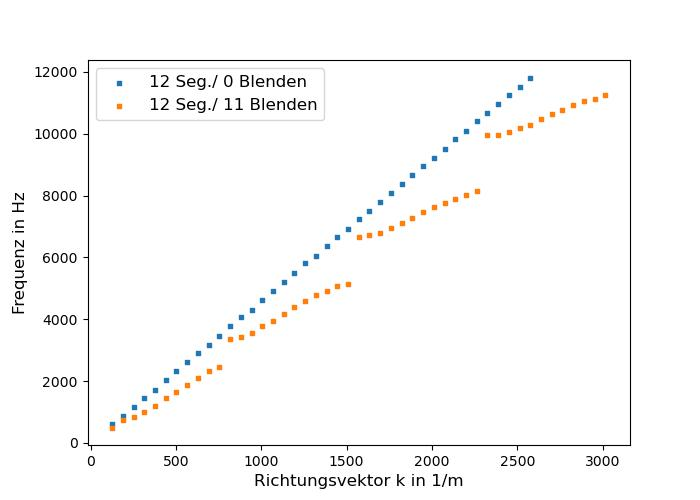
\includegraphics[width=0.8\textwidth]{Bilddateien/Auswertung/V_l_Dispersionsrelation_Kurz.jpg}
            \caption{Dispersionsrelation der Resonanzspektren des Rohrs aus \ref{fig:V_l_Resonanzspektrum_Kurz}, für verschiedene Segment- und Blendenzahlen}
            \label{fig:V_l_Dispersionsrelation_Kurz}
        \end{figure}

        \begin{figure}[H]
            \centering
            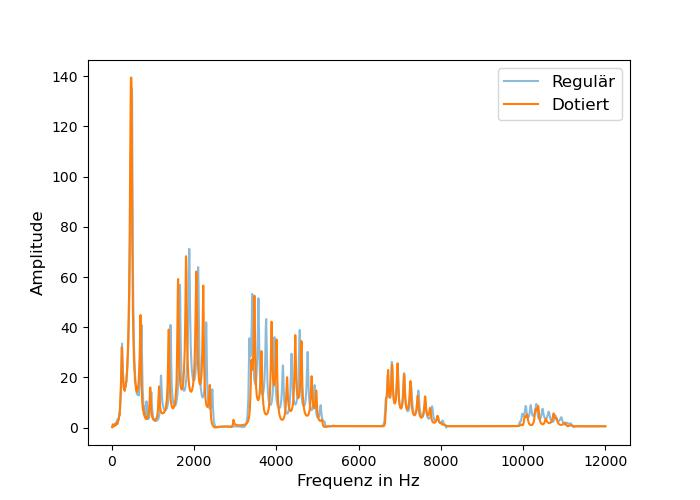
\includegraphics[width=0.8\textwidth]{Bilddateien/Auswertung/V_o_Resonanzspektrum_Dotiert.jpg}
            \caption{Vergleich des Rohrs aus \ref{V_l_Resonanzspektrum_Kurz} (12 Segmente) mit einen, dass 11 kurze Segmente und an der achten Stelle ein Segment der Länge $\SI{75}{\milli\metre}$ hat}
            \label{fig:V_o_Resonanzspektrum_Dotiert}
        \end{figure}

\end{document}